%Preamble
\documentclass[a4paper,12pt]{article}
\usepackage[utf8]{inputenc}
\usepackage{amsmath}
\usepackage{todonotes}
\usepackage{textcomp}
\usepackage{caption}
\usepackage{pdfpages}
\usepackage{chngpage}
\usepackage{hyperref}
\usepackage{comment}
\usepackage{tikz}
\usepackage{braket}
\usepackage{hyperref}
\usepackage{float}
\usepackage{soul}
\usepackage{graphicx}
\usepackage{url}
\usepackage{multirow}
\usepackage{booktabs}
\usepackage{setspace}
\usepackage{dcolumn}
\usepackage{adjustbox}
\usepackage{rotating}
\onehalfspacing
\graphicspath{ {/home/user/images/} }


% Opening
\title{Kidney disease \& Transplantations in Denmark}
\author{Emilie Nordby Lauritzen \& Simon Kjær Bjerg}
\date{20. April 2017}


\begin{document}
\maketitle
\newpage

\begin{abstract}
\end{abstract}	
\newpage
\tableofcontents

\newpage
\section{Introduction}

\subsection{Background}

Living with a kidney disease is a life changing diagnosis that XXX live with in Denmark every year. Even with modern medicine the only cure for kidney disease is receiving a new organ. This reality means that there is a tremendous demand for donor kidneys, a demand that by far is exceeding the supply. Every year XXX dies while on a waiting list for a new kidney. 
\\\\
A lot of papers argue that the current Danish kidney program is inefficient reference and that the amount of donor kidneys could be increased by implementing a donor system. If Denmark were to actually implement a donor kidney system, it would be based on the premise, that kidney transplantations is favored in a socio-economic perspective relative to the patients with a kidney disease just getting dialysis. Based on this argument the paper seeks to perform a Cost Utility Analysis on kidney transplants weighted against the alternative, dialysis.

\subsection{Purpose}

The purpose of this paper is to analyse and compare the possible means of treatment, for individuals living with kidney disease. The paper aims to illuminate the cost and benefits associated with the distinct treatment interventions.
\\\\
To make this comparison, the paper seeks to uncover the price of dialysis and kidney transplantations and on that basis estimate the cost of both interventions. Furthermore we seek to approximate the before mentioned costs, in both a societal and regional perspective. Moreover we will investigate the effect of treatment in a Quality Adjusted Life Year framework, to better understand the associated output in addition to merely considering the costs.


\subsection{Limitations \& assumptions}




\section{Method}

\subsection{Cost Effectiveness Models}

When evaluating if a health program should be implemented or not, three different methods are commonly used; Cost Benefit Analysis (CBA), Cost Effectiveness Analysis (CEA) and Cost Utility Analysis (CUA). The approach and conclusion of the three methods differ, which makes them useful for different kinds of analyses. An effectiveness analysis consists of two parts, the costs and the effects of the intervention. The way the costs are estimated will generally be the same for the three effectiveness analyses, while the measurement of the effect will differ depending on the approach used \cite{Christiansen2010}. In the following we will outline the method for each of the effectiveness analysis above and from this deduct the method we will use in this paper.  
\\\\
The CBA is the least used effectiveness analysis of the three mentioned. A CBA will directly compare the monetary cost and benefit of one or more interventions and will always be conducted from the societies perspective. The CBA makes it easy to compare interventions because it is measured in monetary values, further more the CBA rests on the assumption that an intervention should only be implemented if the extra effectiveness (benefit) exceeds the extra cost of the intervention. (Edlin, McCabe, Hulme, Hall, Wright; 2014)
\\\\
A CEA relies on the assumption that the purpose of an effectiveness analysis should be to maximize what the decision maker would like to maximize. (Edlin, McCabe, Hulme, Hall, Wright; 2014) This means that a CEA only includes what the decision maker finds relevant, which additionally depends on the kind of decision maker, which could be society, public sector, health sector or something completely else. In contrast to a CBA, a CEA is measured in natural units such as Incremental Cost Utility Ratio, number of deaths avoided etc. It is worth to point out that the natural unit should be consistent, which means it cannot change depending on the individual or intervention looked at (Edlin, McCabe, Hulme, Hall, Wright; 2014). 
\\\\
CUA is seen as a sophisticated version of CEA. This is because CUA is utility based, which means the outcome of a CUA takes the patients health state into account opposed to a CEA. This is done by using quality adjusted life years (from now on referenced as QALY). This means that the effectiveness part of the analysis is weighted with how good the individual is feeling, 1 for perfect health, 0 for death. Due to this method we can compare how many QALY’s an intervention will produce compared to not implementing the intervention or implementing another intervention. 

\begin{figure} [h]
	\centering
	\caption{Interpretation of QALY}
	\label{fig:qaly}
	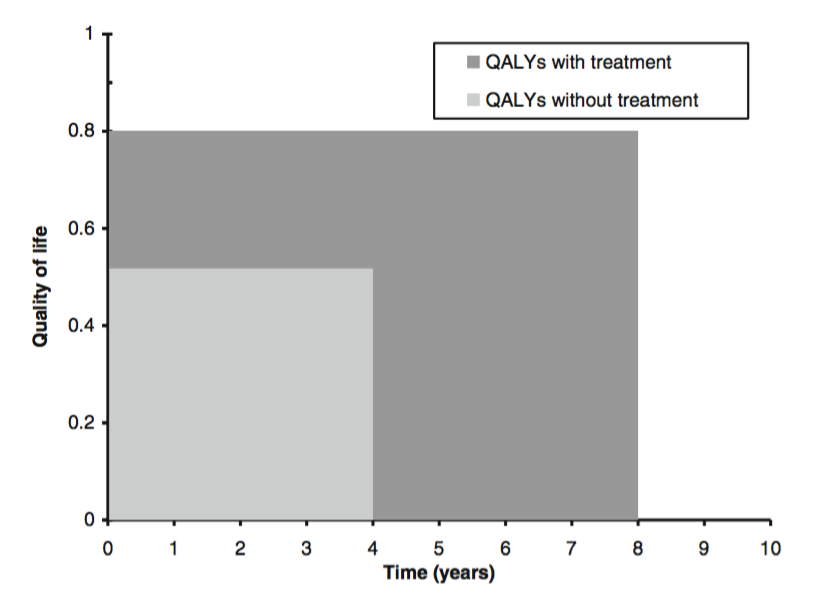
\includegraphics[width=0.7\linewidth]{Pictures/QALY}
	\caption*{Source:  \cite{CUAbog} }
\end{figure}

\subsubsection*{ICER}
When comparing interventions, we would like to know how much better a intervention is against the next best alternative. This is done by using the Incremental cost effectiveness ratio (ICER). The ICER is calculated in the following way: 
\\\\
\begin{equation} ICER=\dfrac{C_2-C_1}{E_2-E_1} =\dfrac{\varDelta C}{\varDelta E}
\end{equation}
\\\\
where $ C_2$ is the cost of the intervention under investigation, $ E_2$ is the effectiveness of the intervention under investigations, $ C_1$ is the cost of the comparison, $ E_1$ is the effectiveness of the comparison. When using a CUA our effectiveness will be in QALY’s and the ICER will reflect the extra cost of one more QALY. This can be plotted in the figure below, where the South Eastern quadrant is seen as dominant, and the intervention of interest should be implemented. 

\begin{figure} [h]
	\centering
	\caption{Plotting of ICER}
	\label{fig:ICER}
	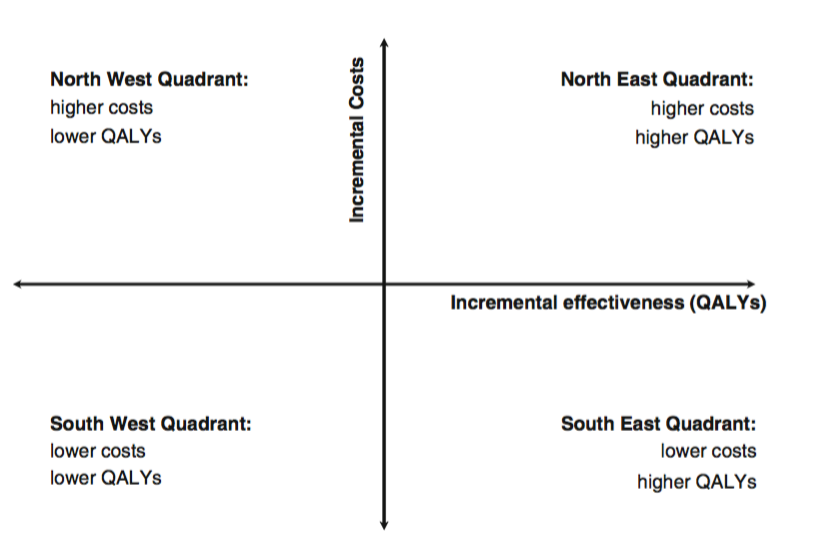
\includegraphics[width=0.7\linewidth]{Pictures/ICER}
	\caption*{Source:  \cite{CUAbog} }
\end{figure}

If results are plotted in the North Western Quadrant, then the alternative intervention will be dominant (the intervention of interest are both more expensive and less effective than the alternative). The last two quadrants (North East and South West) are a little more complicated, and in this case, the decision maker would set a ceiling ratio, which is the level of ICER which the intervention must meet to be cost effective and thereby implemented.   This ceiling is sometimes seen as a willingness to pay, i.e. the willingness to pay an extra QALY. 
\\\\
In this paper, we investigate whether kidney transplantation is cost effective against the alternative, dialysis. As we want to take the quality of the patient’s life into account, we will choose to use a CUA, to compare the two treatments.  

\subsection{Markov Chain model}

The foundation for the Cost Utility Analysis is a Markov Chain model. A Markov Chain is a simple, yet powerful model, which is frequently applied in health economics. The Markov Chain model is used to explore the journey a hypothetical cohort of people can takes through a defined set of states. The journey of a person in the Markov Chain model is based on the probabilities of switching between these states.
\\\\
A Markov Chain is build on the idea that individuals can change between different states, which is defined as Markov states. In our model a Markov State is a specific health state. For any given point in time the individuals in the cohort has to appear in a Markov State, thus there cannot be individuals outside the defined states. Furthermore, the states are required to be mutually exclusive with no overlap allowed. An individual stay in a given health state for a fixed amount of time, a cycle. A cycle can be of any length and covers all the health states, why a cycle is of the same length for every state. At the end of every cycle the hypothetical individual either stay in their current health state or transitions to another.
\\\\
A simple Markov Chain model consisting of 3 health states; Well, disease and dead. A graphic of this simple Markov Chain model can be examined in the influence diagram below.
\\\\
\begin{figure}[h]
	\centering
	\caption[]{Simple Markov model}
	\label{fig:markov-simple}
	\includegraphics[width=0.7\linewidth]{"Pictures/Markov simple"}
	\caption*{Source}
\end{figure}
\\\\
The arrows in the diagram above identifies the possible transitions between states. It is both possible to transition from well to disease and from disease to well, but once an individual has transitioned to dead, the individual is said to have reached an absorbing state. An absorbing state is defined by a 100\% probability of staying in that state and therefore a 0\% probability of transitioning to another state. 
\\\\
The Markov States are tied together through a transition matrix which defines the conditional probability of moving from one Markov State to another, or staying in the current state, conditioned on the current state. The transition matrix is applied at the end of every cycle. The cycles continue for a fixed amount of time or until a specific level of convergence is met. Below the framework for the above illustrated Markov Chain model can be examined.
\\\\
\begin{figure}[h]
	\centering
	\caption[]{Transition matrix}
	\label{fig:transition-matrix}
	\includegraphics[width=0.7\linewidth]{"Pictures/Transition matrix"}
\end{figure}




\subsubsection*{Markov Trace}
Mathematically the Markov Chain model works through matrix multiplication where the cohort is multiplied with the transition matrix for each period in the model. This mathematical framework has the implication of making the model memory free. The memory free model is a simplification which makes the math easier and requires less of the underlying data. The simplification means that the hypothetical cohort is presented with the same transition matrix each period regardless of the previous states, thus the transition probabilities are merely conditional on the current health state, not prior health states. 
\\\\
Initially the desired output of the model is what is known as the Markov Trace. The Markov Trace is the movement of the cohort between Markov States, throughout the timeline of the model. For every period of the model the amount of people in each state is calculated.

\subsubsection*{Prices}
Once the Markov Trace has been calculated the movement of the hypothetical cohort is known. This information allows for the calculation of a given medical intervention’s cost over a given timeframe. The amount of individuals in each state is simply multiplied with the cost associated with every state in a period. Once the price of every period has been calculated the total price for the timeframe of the model is apparent when summing the costs of the individual periods.

\subsubsection*{QALY – Quality Adjusted Life Years}
In what has been described at this point, this entire model has been cost focused, however there is another dimension to the calculation, the return to the encountered cost. In health economics Quality Adjusted Life Years is a common measure of the return to a given medical intervention. QALY measures the burden of disease and ranges from 1 and below. A QALY of 1 indicates full quality of a lived year, whilst a QALY lower than one identifies a life year of lesser quality than that of a life year in perfect health. A QALY of 0 is assigned to the state of being dead, while a QALY lower than 0 indicates a state deemed to be worse than dead. 

\subsubsection*{Time \& Discounting}
The Markov Chain model is heavily depended on time, as cycles is a core element of the model. This implication of time, means that cycle length and time horizon of the model potentially can have a great impact on the model output. The cycle length is determined by the minimum timeframe of a stage. This cycle length is chosen as all stages abide by the same time structure, meaning that all individuals will stay in a given stage for the full length of a cycle. In theory the cycle length can be decided arbitrarily, however in practice the minimum length of a distinct event is often chosen as it makes the analytical work easier. Sometimes events are combined to make more sensible cycle lengths. A hospitalization can easily include a variety of interventions (check of vitals, a scanning etc.) for ease these would typically be grouped together under the label hospitalization to keep a simpler cycle structure. 
\\\\
Previously when discussing the Markov Trace, transition probabilities were of great importance. Analytically it is therefore very important to consider how these probabilities are calculated based on the chosen cycle length.
\\\\
Once the cycle length has been determined based on sensible arguments, the time horizon of the model has to be determined. The time horizon determines the amount of periods or cycles the model is run for. The time horizon needs to be meaningful in relation to the analysis at hand, meaning that it needs to run long enough to capture both short term and long term effects of a given intervention. The typical time horizon for health analysis is the expected lifetime of the sample in question. Sometimes the time horizon will differ from the expected lifetime for a variety of reasons. One reason could be a preference from the decision maker and the receiver of the analysis. A governmental budget might be available on a two-year horizon, why the analysis might be required to run for the same timeframe. 
\\\\
Lastly in relation to time it is also beneficial to think about when a given cost and benefit is encountered. Therefore, it is the norm to implement a discount rate to establish a consistent measure of cost and benefits. A discount rate is typically chosen based on country standards for the specific analysis at hand.


\section{Costs}
The CUA will both include direct and indirect costs. The direct costs are the costs directly linked to the treatment, where the indirect costs consider for example lost labor, early retirement etc.   Other papers have only looked at the direct costs \cite{CUAdkartikel}, but this does not take all of the relevant costs into account, as an early retirement can be the difference between being a net contributor or net gainer when it comes to public  benefits.  We there fore extend the analysis to take the indirect costs into account as well. 

\subsection{Direct Costs}
There are several costs linked to having a kidney disease. These costs are identified by using the Danish diagnose–related groups (DRG) tariffs and the Danish Ambulatory Groups System (DAGS) that represent the average public health-care cost for patient treatments and ambulatory visits \cite{takst}. All costs are in 2016 DKK prices so we can compare.
\\\\
DNSL!!!!!!!!

\subsubsection*{Dialysis Costs}

 In regards to dialysis, there are as mentioned two different kinds the patient can choose between, P-dialysis and hemodialysis. The split between patients receiving P-dialysis and hemodialysis is 21,1\% and 78,9\% respectively \cite{DNSL} (evt fodnote omkring hvordan, det er fundet). Hemodialysis performed on a hospital requires 3 treatments a week. If the Hemodialysis is performed at home, a check-up every second month is required \cite{Rigshospitalet}.  
 \\\\
 P-dialysis are almost always performed at home (99\% of the time \cite{DNSL}), and we will assume that all patients getting P-dialysis, are doing the treatment at home. P-dialysis gives the patients more freedom and the patient can basically decide for themselves how often they would like to perform the dialysis. Even though the procedure for P-dialysis can differ, the patient needs to go to a check-up on the hospital every 6th week, furthermore there is a cost linked to training the patient to be able to carry out the dialysis at home \cite{P-dialyse}. 

<<<<<<< Updated upstream
\subsubsection*{Tranplantation Costs}

When receiving a kidney, the kidney will either come from a living og deceased donor. In Denmark the share of kidneys recieved from deceased donors are 57,5\% whereas the share of kidneys received from a living donor is  42,5\% \cite{DNSL}. A deceased donor is assumed to donate 3,3 organs, and the price of the kidney donation from a living donor  is therefore divided by 3,3 to get the cost of getting a kidney from a deceased donor. 
\\\\
The biggest cost in relation to a kidney  transplantation is the actual surgery. The surgery is divided into two types; a complicated and a normal kidney transplantation. The probability of undergoing a complicated surgery is 11\%, whereas the probability of a normal surgery is 89\% \cite{esundhed} \cite{CUAdkartikel}. After having a kidney transplantation, the patient should go to a check up 2-3 times a week in the preceding year after the operation. If there is no complications the patient can go to check-ups every other month the following years \cite{Rigshospitalet}. 
\\\\
Another cost linked to a kidney transplant is if the transplantation is not succesful which means the kidney either undergoes graft failure or gets rejected. The probability of rejection is 18,5\% \cite{Rigshospitalet}, while the probability of graft failure is 4,9\% \cite{DNSL}. In this case, the patient will have to get dialysis.

\subsection{Indirect Costs}
=======





\section{Tabeller}



% latex table generated in R 3.2.2 by xtable 1.8-2 package
% Thu Apr 20 15:05:04 2017
\begin{adjustbox}{center}

	\centering
	\begin{tabular}{llrrrr}
		\hline
		Type & Procedure & Cost & Freq. & Weight & Yrl. Price \\ 
		\hline
		HD & At hospital & 1946.00 & 156.00 & 0.93 & 282325.68 \\ 
		HD & At home check up & 21773.00 & 6.00 & 0.07 & 9144.66 \\ 
		HD & Change to peritonal dialysis & 13111.00 & 1.00 & 0.03 & 413.00 \\ 
		HD & Mortality & 0.00 & 1.00 & 0.19 & 0.00 \\ 
		PD & At home  & 1695.00 & 156.00 & 1.00 & 264420.00 \\ 
		PD & Home check up & 20484.00 & 8.67 & 1.00 & 177528.00 \\ 
		PD & Change to haemodialysis & 16818.00 & 1.00 & 0.21 & 3521.69 \\ 
		PD & Mortality & 0.00 & 1.00 & 0.16 & 0.00 \\ 
		Transplantation & Deceased donor & 11034.11 & 1.00 & 0.63 & 6951.49 \\ 
		Transplantation & Living donor & 55896.60 & 1.00 & 0.37 & 20681.74 \\ 
		Transplantation & Transplantation, complicated & 540685.00 & 1.00 & 0.11 & 59475.35 \\ 
		Transplantation & Transplantation, normal & 257992.00 & 1.00 & 0.89 & 229612.88 \\ 
		Transplantation & Check-up & 1382.00 & 12.75 & 1.00 & 17620.50 \\ 
		Transplantation & Payment by patient  & -3955.00 & 1.00 & 1.00 & -3955.00 \\ 
		Transplantation & Rejection & 41509.00 & 1.00 & 0.18 & 7471.62 \\ 
		Transplantation & Graft Failure & 41509.00 & 1.00 & 1.00 & 41509.00 \\ 
		Transplantation & Change to p-dialysis & 13111.00 & 1.00 & 0.04 & 519.20 \\ 
		Transplantation & Change to h-dialysis & 16818.00 & 1.00 & 0.17 & 2820.38 \\ 
		Transplantation & Mortality & 0.00 & 1.00 & 0.03 & 0.00 \\ 
		Transplantation & (Sandimmum Neoral) & 25.08 & 730.00 & 1.00 & 18308.40 \\ 
		Transplantation & (Cellcept) & 23.26 & 730.00 & 1.00 & 16979.80 \\ 
		Transplantation & (Prednisolon) & 2.99 & 730.00 & 1.00 & 2182.70 \\ 
		Transplantation & Indirekte omkostning & 255438.55 & 1.00 & 1.00 & 255438.55 \\ 
		Transplanteret & Indirekte omkostning & 200253.55 & 1.00 & 1.00 & 200253.55 \\ 
		HD & Indirekte omkostning & 276441.49 & 1.00 & 1.00 & 276441.49 \\ 
		PD & Indirekte omkostning & 231238.03 & 1.00 & 1.00 & 231238.03 \\ 
		Dead & Indirekte omkostning & 356475.15 & 1.00 & 1.00 & 356475.15 \\ 
		\hline
	\end{tabular}

\end{adjustbox}
>>>>>>> Stashed changes


\newpage
\begin{thebibliography}{9}

\bibitem{metodebog}
Metodebog

\bibitem{Christiansen2010}
Christiansen; 2010

\bibitem{CUAbog}
CUA bog

\bibitem{CUAdkartikel}
In dk .... 

\bibitem{takst}
Takstvejledning 2016

\bibitem{Rigshospitalet}
Rigshospitalet om nyre

\bibitem{P-dialyse}
P-dialyse

\bibitem{esundhed}
Esundhed

\bibitem{DNSL}
DNSL

\end{thebibliography}	
	

\end{document}






